\section{Partie 1}

\subsection{Cross-Validation with GridSearchCV}
\textbf{{Question}: Explain in your report what happens when we run clf.fit(X\_train, Y\_train). What is the complexity for each of the three following cases?} \\
The line clf.fit(X\_train, Y\_train) here uses the fit method on the object  clf and taking the train sample. We give the features X and the outputs Y. The object clf is from the class GridSearchCV which allows us to find the best hyperparameters among a list we chose. It is taking as parameter an object named knn of the class KNeighborsClassifier(), a dictionary named parameters containing the number of neighbors to be tested in the knn algorithm (1 to 5 here) and the cv parameter referring to the number of folds to be used in the cross-validation. Basically it will perform a 3-folds cross-validation on a kNN model with 1 to 5 neighbors on the train sample and it will allow us to keep the best model. The kNN algorithm is parametered with the default metric which is the Euclidean distance : $\sqrt{\sum^n_{i=1}(x_i - y_i)^2}$. The functions are all part of the sklearn package. \\
Complexity can be divided into two kinds of complexity i.e: 1) time complexity, deal with how long the algorithm is executed, and 2) space complexity, deal with how much memory is used by it's algorithm.\\
\begin{table}[ht]
		\caption{Complexity}
		\vspace{0.5cm}
		\centering
		\begin{tabular}{|c|c|c|c|c|c|c|c|}
			\hline
			& kNN & Linear SVC & Log Reg   \\  [0.3ex]
			\hline 
			Time Training    & O(n*k*d)       &  O(m*n)     & O(n*d)        \\ 
			\hline 
			Space  &  O(n*d)      &       &  O(d)      \\ 
			\hline 
		\end{tabular} 
        \label{table:nonlin}
	\end{table}	

With n : size of the training sample, d : dimension of the data, k : number of neighbors and m : number of features

\textbf{{Question}:What is the test accuracy? What would be the accuracy of random guess?} \\
The test accuracy is the measure of how often the points are correclty classified. In our case the accuracy is 0.875.  It means that 87.5\% of the time, the points are correctly classified on the test sample. If we did a random guess we would randomly choose an output in the range 0 to 9 so the accuracy would converge towards $\frac{1}{10}$ according to the LLN.  \\


\textbf{{Question}:  What is LinearSVC() classifier? Which kernel are we using? What is C? (this is a tricky question, try to find the answer online )}\\
LinearSVC means Linear Support Vector Classification, which is supervised learning methods used for classification. LinearSVC are classes capable of performing binary and multi-class classification on a dataset. 
This classifier tries to find a line that separates the True labels from the False labels.. We are using a linear kernel. The parameter C represents the regularization weights, ie the penalty applied on the loss function. The loss function used here is the Squared Hinge Loss : $l(y)=\max(0,1-t\cdot y)$ \\
\todo{Add description of SVC}


\begin{figure*}[ht]
	\centering 
	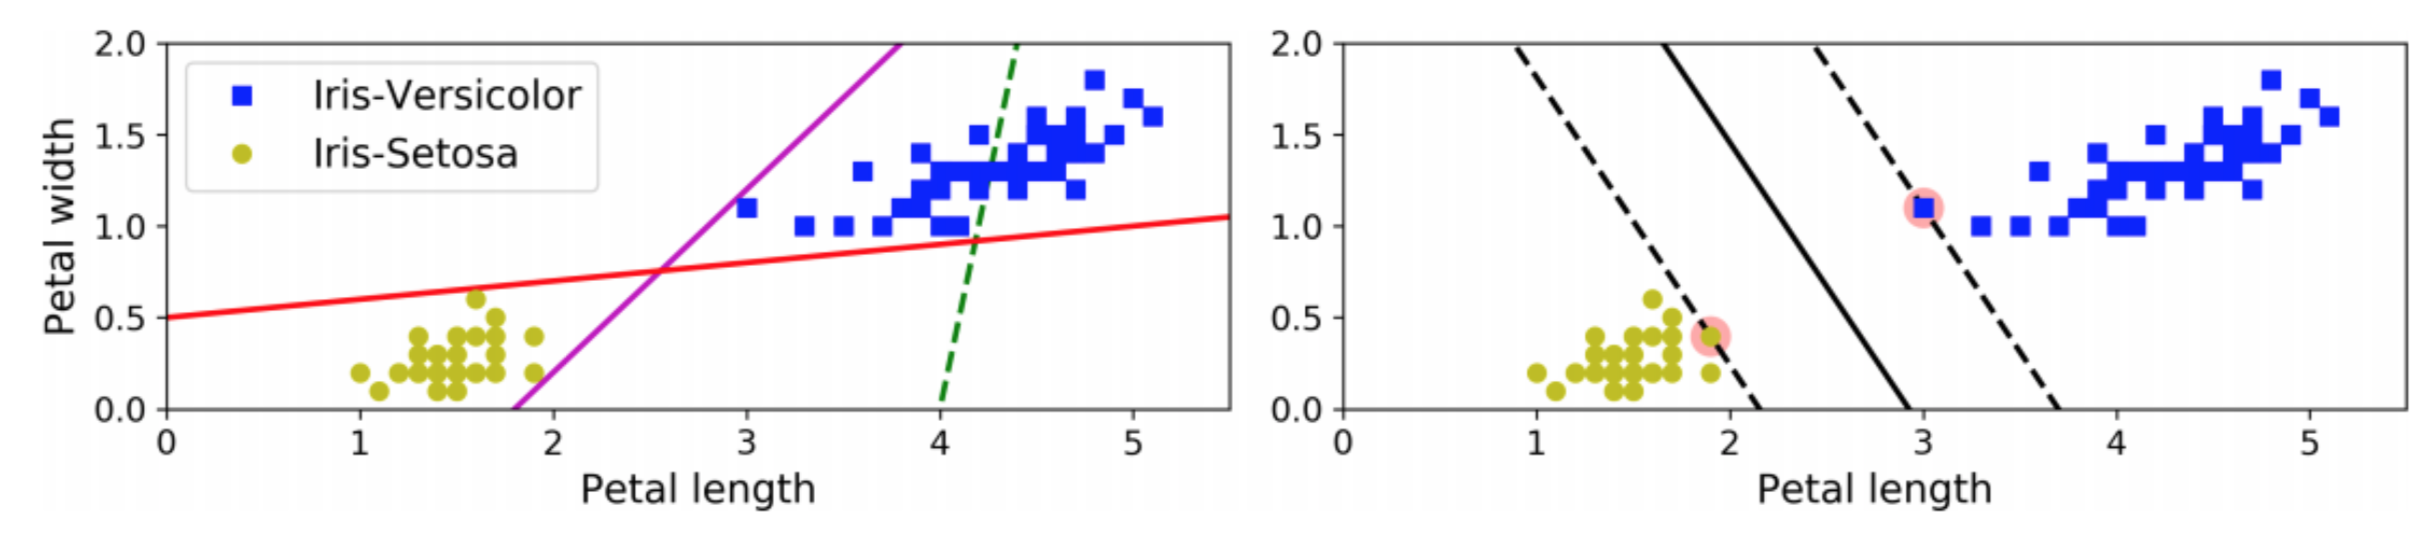
\includegraphics[scale = 0.35]{Pics/SVM}
	\label{fig:svmex}
\end{figure*}

\textbf{{Question} : What is the outcome of np.logspace(-8, 8, 17, base=2)? More generally, what is the outcome of np.logspace(-a, b, k, base=m)?}\\
The outcome of np.logspace(-8, 8, 17, base=2) is a logarthmic space going from $2^{-8}$ to $2^8$ with 17 numbers equally spaced on log scale.
 The logspace function from the numpy package will return k numbers going from $m^{-a}$ to $m^b$ spaced on a log scale with a log base m. \\

\textbf{Question : What is the meaning of the warnings? What is the parameter responsible for its appearence?}\\
The warning tells us that the algorithm did not converge, it did not reach the stop criterion. The parameter responsible for its appearence is the max\_iter parameter. Its value is not sufficient for the algorithm to converge. The data variance is maybe too large for the algorithm to efficiently perform the SVM. \\

\textbf{Question : What did we change with respect to the previous run of LinearSVC()?} \\
We are running the svc function which is by default a RBF SVC and not a linear SVC. RBF means radial basis function. We added a parameter MaxAbsScaler() to scale the absolute data between 0 and 1 and thus reduce the variance. \\

\textbf{Question : Explain what happens if we execute} 
\begin{verbatim}pipe.fit(X_train, y_train)
pipe.predict(X_test, y_test)\end{verbatim} \\
Those lines will execute the pipeline defined with a \verb|MaxAbsScaler|  preprocessing on the features and a SVM algorithm but with no C parameter defined which will be 1.0 by default.\\

\textbf{Question : what is the difference between} \verb|StandardScaler()| and \verb|MaxAbsScaler()|? \textbf{What are other scaling options available in sklearn? }\\
StandardScaler will normalize the data : $\frac{x-m}{\sigma}$ with m the mean and $\sigma$ the standard deviation of data. It differs from StandarScaler because absolute values are mapped in the range [0,1]. \\
The other scaling option available in sklearn are : \\
- \verb|MinMaxScaler| which transform features by scaling each feature to a given range, \\
- and \verb|RobustScaler|, this scale is used if your data contains many outliers. \\ 
\todo{Add other options for scaling}

\textbf{Question : Using the previous code as an example achieve test accuracy  $\geq0.9$ . You can use any method from sklearn package. Give a mathematical description of the selected method. Explain the range of considered hyperparamers.}\\
We tried the Random Forest algorithm which is \todo{definition of random forest mathematically}. We used a pipeline with a scaler : the standard scaler to have less variance in the data and the \verb|RandomForestClassifier()| function from the skLearn package. The hyperparameters tested are the number of trees to estimate, we chose 100 (default) and 150,  and the variance criterion used in each tree to select a feature and a threshold, entropy or gini coefficient.


\subsection{Visualizing errors}
The error in the chunk of code was because the \verb|predict_proba| method returns an array of probabilities within an array. We must then pick the first element of the array (index 0) to obtain the proabilities array (see line 11 appendix \ref{appendix:visualizing}).\\

\subsection{Changing the loss function}
 
\textbf{Question: What is balanced\_accuracy\_score? Write its mathematical mathematical description.} \\

The balanced accuracy in binary and multiclass classification problems is used to deal with imbalanced datasets. 
It is defined as the arithmetic mean of the sensitivity (also called recall or true positive rate) and the specificity (also called true negative rate). As a consequence, it represents the average accuracy per class.
recall = TP/(TP + FN) TP: true positive and FN: false negative
specificity = TN/(TN+ FP)
Instead of calculing the regular score which is (TP+TN)/all predictions, the balanced score is (recall+specificity)/2. If the number in each categorie of prediction is the same, regular score= balanced score. Otherwise, the good predictions of an over represented class will not inflate the balanced score unlike the regular one.\\

balanced\_accuracy\_score is a method from the sklearn package that computes the balanced accuracy metric. 


In classification, the accuracy is the percentage of well-classified individuals on a test sample. The formula is : \begin{equation*}
True Positive + 	True Negative \over Sample Size
\end{equation*}
But this metric does not take into account if the sample is imbalanced. For example if we have more real positives than real negatives. The balanced accuracy takes this into account by taking the average value of true positives divided by real positives and true negatives divided by real negatives as follows : \begin{equation*} \frac{tp}{rp}+ \frac{tn}{rn} \over 2
\end{equation*} \\

\textbf{Question: What is the confusion matrix? What are the conclusions that we can draw from the} \verb|confusion_matrix(y_test, clf4.predict(X_test))?| \\

The general idea is to count the number of times instances of class A are classified as class B. For example, to know the number of times the classifier confused images of 5s with 2s, you would look in the 5th row and 2nd column of the confusion matrix. In row the actual class and in columns the predicted class given by algorithm. \\

As we can see, in figure \ref{fig:confusion}, appendix \ref{appendix:changingloss}, 8s are often confused with 5s (3/17=18\% of the time when the actual class is 8) and 3s are also confused with 5s 13\% of the time (3/23). Also, 5s are detected only 57\% (8/14) of the time. 0s and 9s seem well detected with respectively 100\% (22/22) and 92\% (24/26) recall/true positive rate.\\

Regarding the scores, the balanced is slightly inferior to the regular one (83\% vs 84\%) due to the underrepresentation of the worst predicted class (ie 5s).Because there are several class, it could be interesting to transform the confusion matrix into a heat map. \\

On the heat map we can check that the algorithm is pretty good at predicting classes since most images are on the main diagonale. Even though, 5s are darker than other classes explained by the underrepresnetation of the class and the lower number of good predictions. 1s are well predicted given its bright square on the main diagonale but it can be partly explained by the overrepresentation of 1s in the datatset. 


